
\chapter{FLOWPAK: Flow-based Ornamental Element Packing}

\mynote{Chapter title too long --> https://tex.stackexchange.com/questions/335346/addcontentslinetoc-with-a-linebreak-or-newline-for-the-toc}



\section{Introduction}

\begin{figure}[ht] %%% ELEMENT IMAGE
\centering
\includegraphics[width=0.6\textwidth]{figures/flowpak/dog_ornament_flow.pdf}
\vspace*{-8pt}
\caption{
  \label{dog_flow}
  An example of flow visual style, 
  including a visualization of the flow directions
of elements (by ComicVector703 on Shutterstock).
}
\end{figure}

FLOWPAK~\cite{Saputra2017} is a technique for filling a container 
region with elements that are deformed 
to communicate a sense of directionality or flow.
Elements can be oriented in the local direction 
of flow, but can also be deformed to capture changes in flow direction.
Flow adds visual interest to a composition,
engaging the viewer by providing a sense of progression and
movement through elements.
A hand-drawn dog example in Fig.~\ref{dog_flow} shows many elements that appear to flow
outward from the flower in the centre of the torso, and then
up the neck and down into the legs.
Although there has been a moderate amount of past research on
the generation of packings or mosaics,
this past work is not appropriate for creating flow-like
designs similar to the dog example.

\section{Previous Work}
\section{Problem Formulation}
\section{Approach}

\begin{figure}
\centering
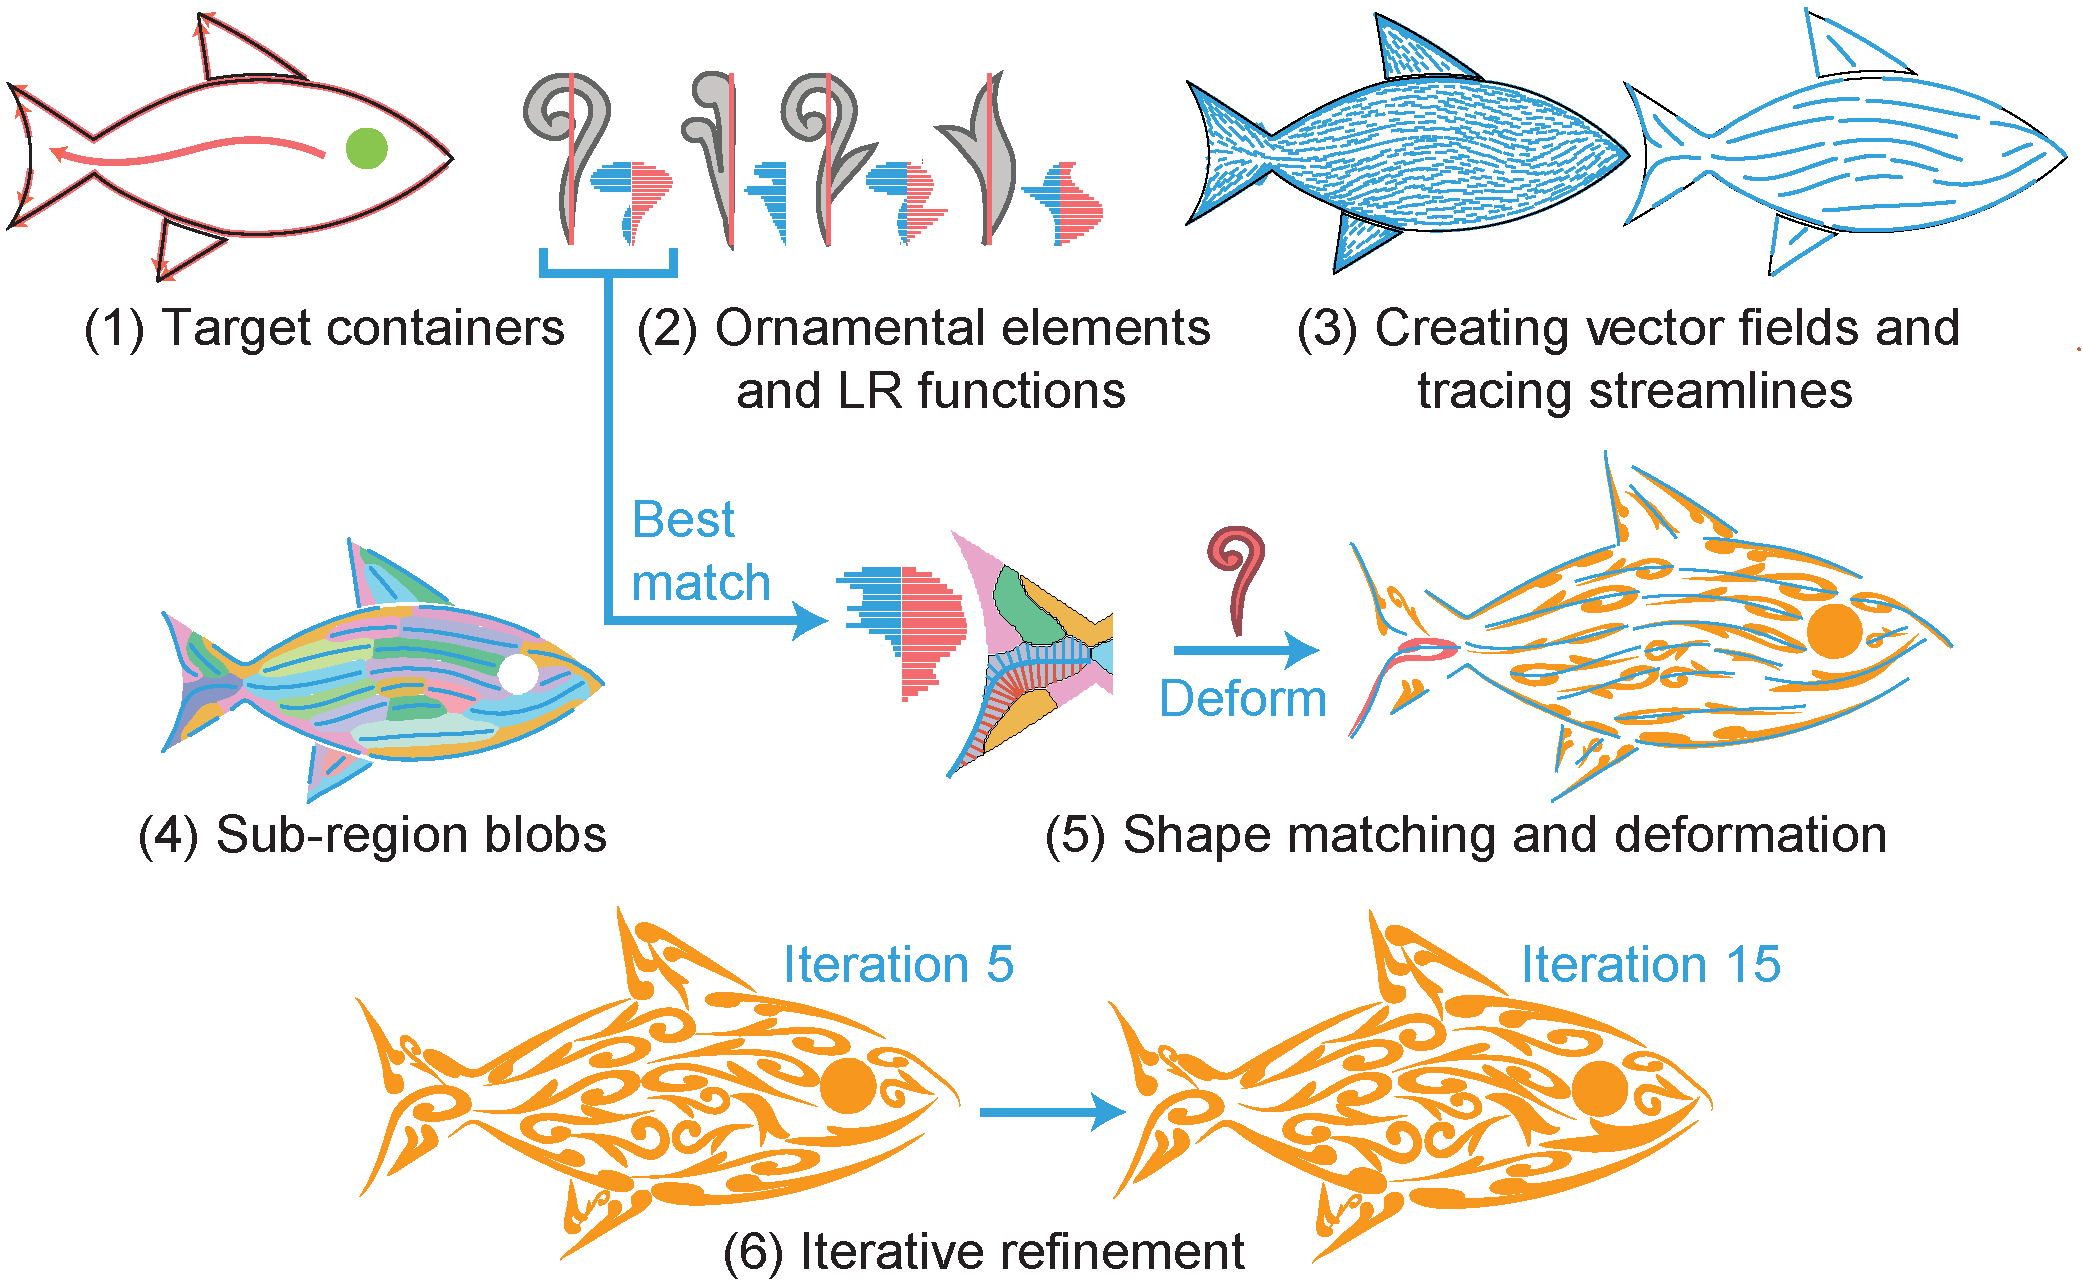
\includegraphics[width=1.0\textwidth]{figures/flowpak/pipeline.pdf} 
\caption{\label{fig_flowpak_pipeline} 
FLOWPAK pipeline. \mynote{Need rearrange}.}
\end{figure}

\subsection{Target Containers}
\subsection{Ornamental elements and LR functions}
\subsection{Creating Vector Fields and Tracing Streamlines}
\subsection{sub-region blobs}
\subsection{Shape Matching and Deformation}
\subsection{Iterative Refinement}
\section{Implementation and Results}

\begin{figure}
\centering
\includegraphics[width=1.0\textwidth]{figures/flowpak/lion_unicorn.pdf} 
\caption{\label{fig_lion_unicorn} 
Lion Unicorn. }
\end{figure}



\section{Conclusions}